\section{Power analysis}
\label{sec:power}

In this section, we'll calculate the variance of our different annotation schemes.

\newcommand{\xh}{\hat{x}}
\newcommand{\xb}{\bar{x}}
\newcommand{\yh}{\hat{y}}
\newcommand{\yb}{\bar{y}}
\newcommand{\rh}{\hat{r}}
\newcommand{\ph}{\hat{p}}

Let $\sC$ be a corpus (our ``population'') that we wish to compute statistics over
and $\sP$ be the population of pooled contexts, 
  with $r \eqdef \Pr(c \in \sP \given c \in \sC)$ (the recall of the pool).

Let $E$ be a randomly drawn subset of $\sC$ with $n_E$ samples for exhaustive annotation and
    $P$ be a randomly drawn subset of $\sP$ with $n_P$ samples for pooling annotation.

\begin{figure}
  \begin{subfigure}{0.49\textwidth}
    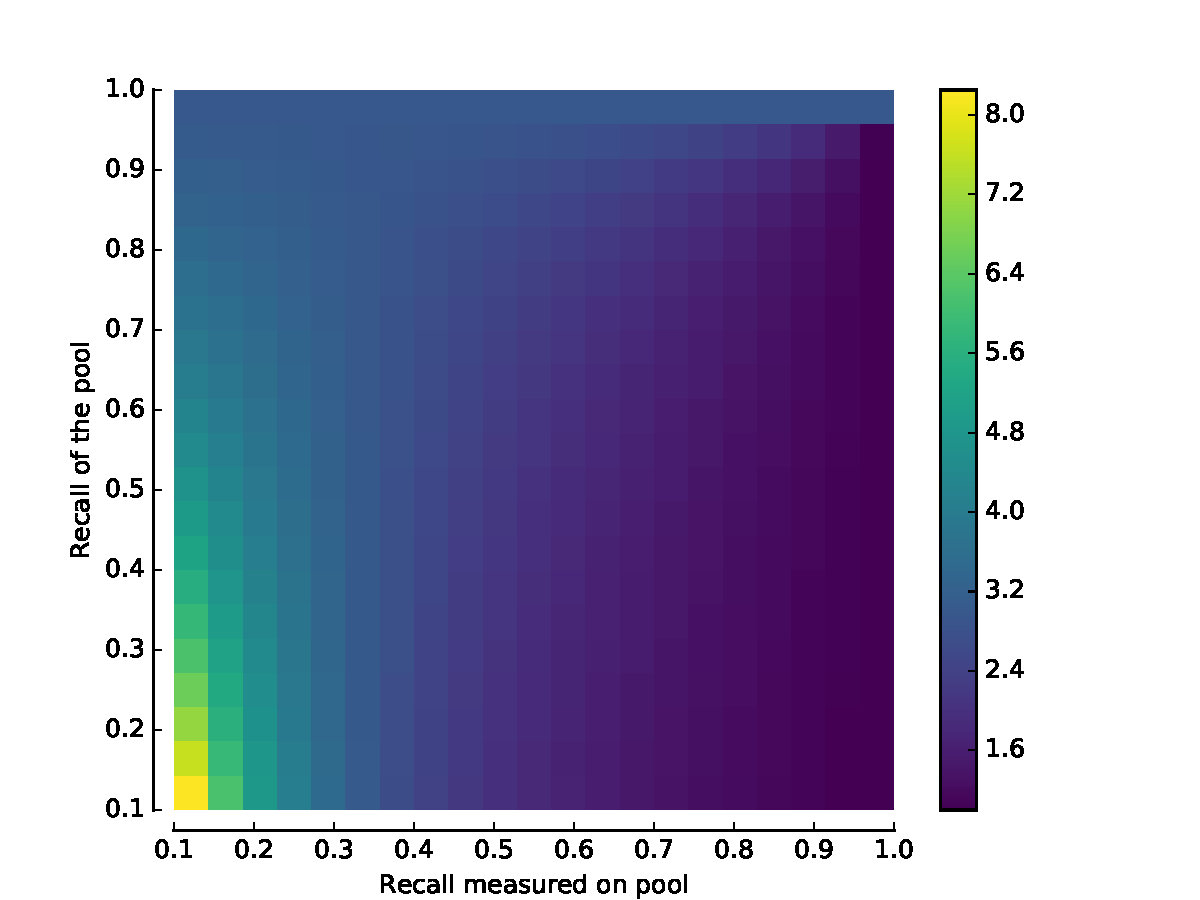
\includegraphics[width=\textwidth]{figures/variance-ratio-pool}
    \caption{\label{fig:pool-for-corpus} The relative efficiency of using pooled annotations versus exhaustive annotation, assuming that there are twice as many pooled annotations as there are exhaustive annotations.}
  \end{subfigure}
  \hfill
  \begin{subfigure}{0.49\textwidth}
    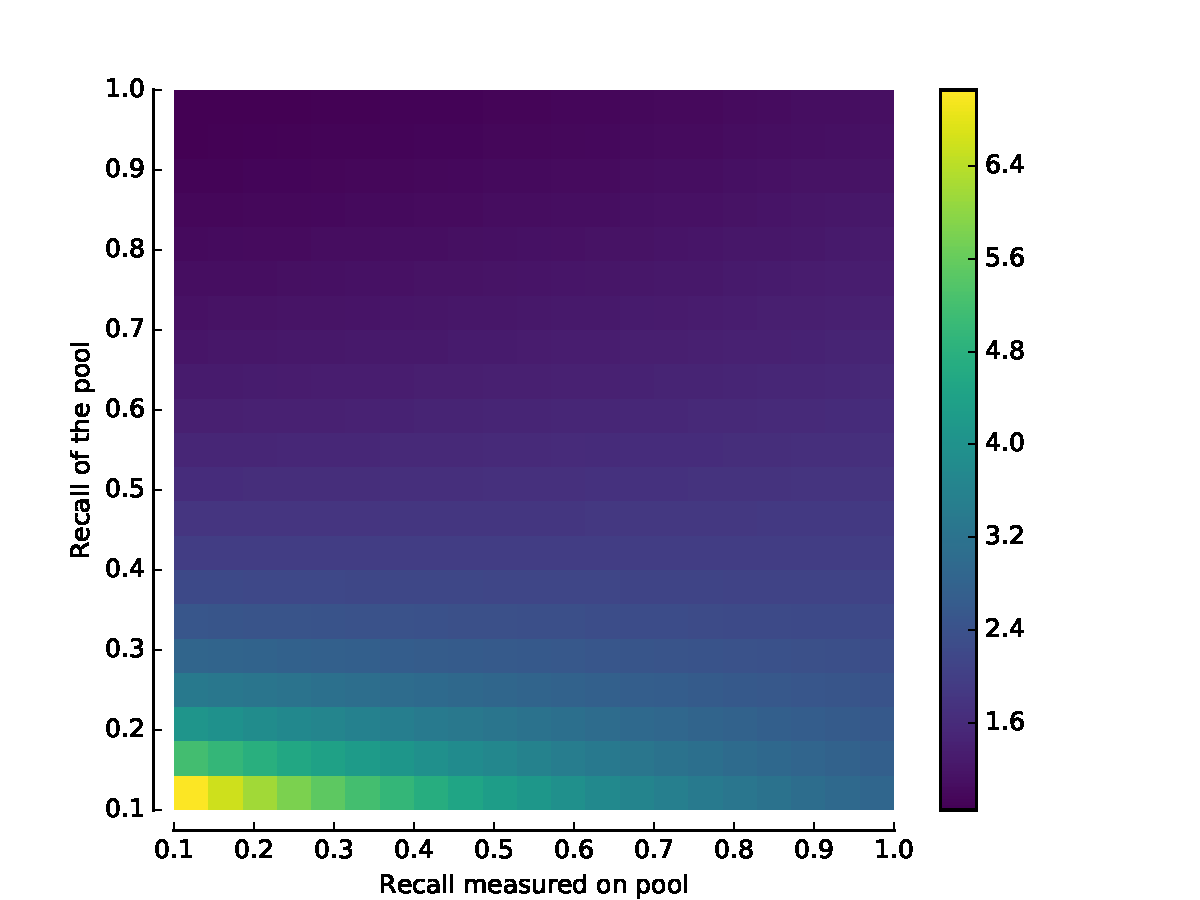
\includegraphics[width=\textwidth]{figures/variance-ratio-unassessed}
    \caption{\label{fig:pool-for-unassessed} The relative efficiency of using unassessed annotations versus exhaustive annotation, assuming that there are twice as many pooled annotations and ten times as many unassessed contexts as there are exhaustive annotations.}
  \end{subfigure}
\end{figure}

\begin{theorem}[Relative efficiency of using pooled annotations to compute corpus statistics] 
  \label{thm:variance-pooled-recall}
  % Define all the variables
  Let $x$ be a statistic that we wish to compute on $\sC$ (e.g.\ recall),
    $\rh$ be an unbiased estimator of $r$ on $E$ with variance $\sigma_r^2$,
    $\yh_p$ be an unbiased estimator of $x$ on $P$ with variance $\sigma_y^2$,
  then $\xh_p = \rh \yh_p$ is an unbiased estimator of $x$ on $P$ with variance
  $$
  \sigma_p^2 = \sigma_r^2 \sigma_y^2 + y^2 \sigma_r^2 + r^2 \sigma_r^2.
  $$

  Furthermore, if $\xh_e$ be an unbiased estimator of $x$ on $E$ with variance $\sigma_e^2$,
  the relative efficiency of $\xh_p$ with respect to $\xh_e$ is,
  \begin{align*}
  \frac{\sigma_e^2}{\sigma_p^2}
  &\approx \frac{1-x}
      {
      y (1-r) + \frac{n_E}{n_P} r (1-y)
      }.
  \end{align*}
\end{theorem}
\begin{proof}
  \begin{align*}
    \sigma_e^2 &= \frac{x (1-x)}{n_E + 1} \\
    \sigma_r^2 &= \frac{r (1-r)}{n_E + 1} \\
    \sigma_y^2 &= \frac{y (1-y)}{n_P + 1} \\
    \sigma_p^2 
    &\approx y^2 \frac{r (1-r)}{n_E + 1} + r^2 \frac{y (1-y)}{n_P + 1} \\
    &= x^2 \left( \frac{(1-r)/r}{n_E + 1} + \frac{(1-y)}{n_P + 1} \right).
  \end{align*}
\end{proof}

\begin{lemma}[Benefit of combining estimators]
  Let $x_1, \dots, x_n$ be independent and unbiased estimators for a statistic $x$ with variances $\sigma_1^2, \dots \sigma_n^2$.
  Let $z = \sum_{i=1}^n \alpha_i x_i$ where $\sum_{i=1}^n \alpha_i = 1$ be a combined estimator for $x$ with minimal variance.
  Then, the relative efficiency, i.e ratio of variances, of $z$ and $x_1$ is,
  $\frac{\sigma_z^2}{\sigma_1^2} = \sum_{i=1}^n \frac{\sigma_i^2}{\sigma_1^2}$.

  In other words, relative efficiency of a combined estimator with respect
  to an original estimator is the sum of relative efficiencies of each component
  estimator with respect to the original estimator. 
\end{lemma}


